\documentclass[conference]{IEEEtran}
\IEEEoverridecommandlockouts
% The preceding line is only needed to identify funding in the first footnote. If that is unneeded, please comment it out.
\usepackage{cite}
\usepackage{amsmath,amssymb,amsfonts}
\usepackage{algorithmic}
\usepackage{graphicx}
\usepackage{textcomp}
\usepackage{xcolor}
\def\BibTeX{{\rm B\kern-.05em{\sc i\kern-.025em b}\kern-.08em
    T\kern-.1667em\lower.7ex\hbox{E}\kern-.125emX}}
\begin{document}

\title{Counterfeit Fingerprint Detection of Outbound HTTP Traffic with Graph Edit Distance}

\author{\IEEEauthorblockN{1\textsuperscript{st} Given Name Surname}
\IEEEauthorblockA{\textit{dept. name of organization (of Aff.)} \\
\textit{name of organization (of Aff.)}\\
City, Country \\
email address}
\and
\IEEEauthorblockN{2\textsuperscript{nd} Given Name Surname}
\IEEEauthorblockA{\textit{dept. name of organization (of Aff.)} \\
\textit{name of organization (of Aff.)}\\
City, Country \\
email address}
}

\maketitle

\begin{abstract}

We present DECANTeR, a system to detect anomalous outbound HTTP communication, which passively extracts  fingerprints for each application running on a monitored host. The goal of our system is to detect unknown malware and backdoor communication indicated by unknown  fingerprints extracted from a host’s network traffic. We evaluate a prototype with realistic data from an international organization and datasets composed of malicious traffic. We show that our system achieves a false positive rate of 0.9\% for 441 monitored host machines, an average detection rate of 97.7\%, and that it cannot be evaded by malware using simple evasion techniques such as using known browser user agent values. We compare our solution with DUMONT [24], the current state-of-the-art IDS which detects HTTP covert communication channels by focusing on benign HTTP traffic. The results show that DECANTeR outperforms DUMONT in terms of detection rate, false positive rate, and even evasion-resistance. Finally, DECANTeR detects 96.8\% of information stealers in our dataset, which shows its potential to detect data exfiltration.

\end{abstract}

\begin{IEEEkeywords}
Anomaly Detection, Data Exfiltration, Data Leakage, Application Fingerprinting, Network Security
\end{IEEEkeywords}

\section{Introduction}

Nowadays, malware usually uses HTTP protocol to connect suspicious host for data leakage and exfiltration, because it's a common network channel that Intrusion Detection/Prevention Systems (IDS/IPS) never block the HTTP traffics. Therefore, malware tries to hide their penetrations in the HTTP traffic to evade the detections in Figure ~\ref{fig:attack}. In the previous research, there are many botnet using HTTP protocl to communicate with the C\&C server for waiting command instead of IRC channel \cite{gu2008botsniffer}. However, the proposed method in the past that uses fingerprint to detect malware hide in outbound HTTP traffics \cite{bortolameotti2017decanter}, and which can't efficiently detect malware when hacker generates counterfeit fingerprints.  

The main idea concept of fingerprint is around the HTTP headers. But, as we know, hacker can use exploit tool or library to eaily modify the contents of a HTTP header. Previous research also indicates that malware uses modified HTTP header to evade the latest detections system \cite{grill2014malware}, and which points out most malware using browser-like user-agent since browser's connection behavior is various and complex. Therefore, we represent the problem define as following:

\begin{figure}[!t]
\centering
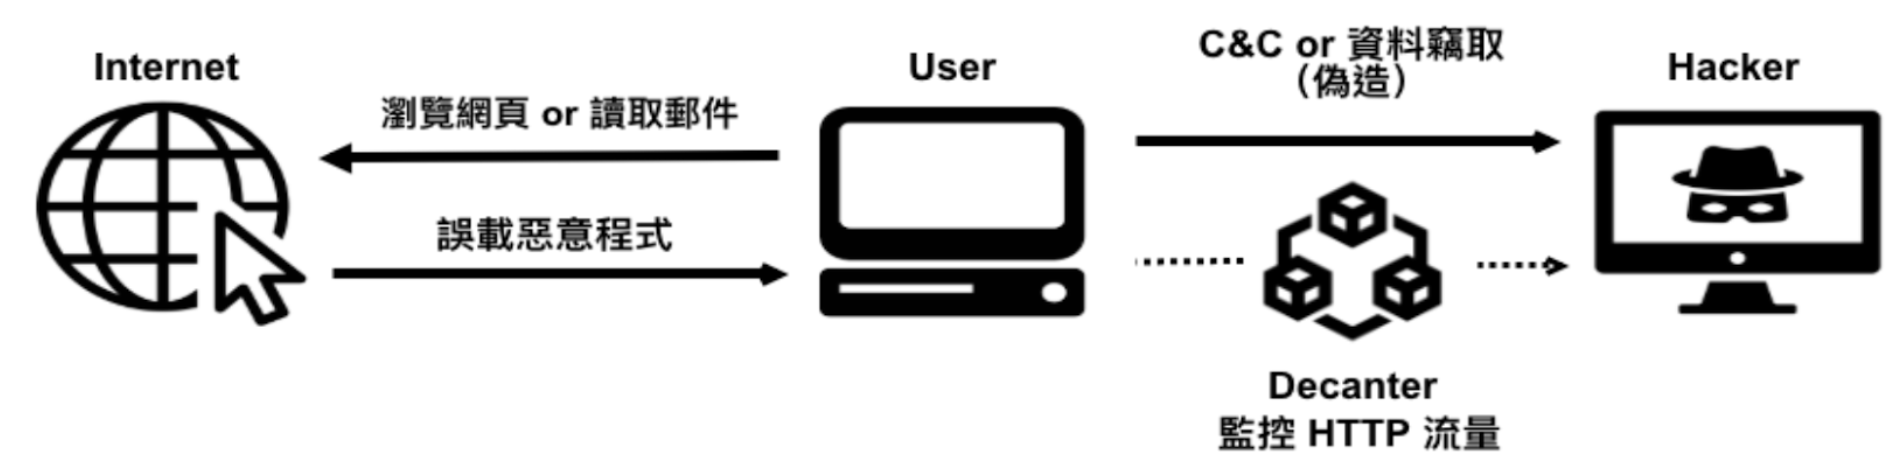
\includegraphics[width=250pt]{image/attack.png}
\caption{A process of attacking scenario}
\label{fig:attack}
\end{figure}


\begin{figure}[!tbp]
  \centering
  \subfloat[Normal Referrer Correlation Graph]{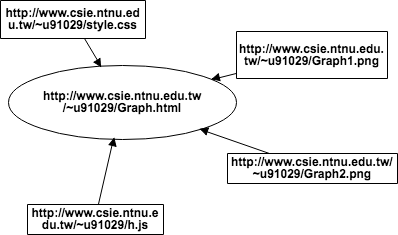
\includegraphics[width=0.25\textwidth]{image/normal.png}\label{fig:normal}}
  \hfill
  \subfloat[Malicious Referrer Correlation Graph]{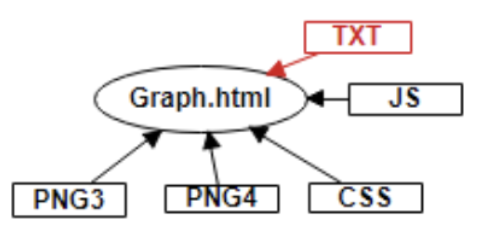
\includegraphics[width=0.25\textwidth]{image/malware.png}\label{fig:malware}}
  \caption{Difference between normal and malicious referrer correlation graph.}
\label{fig:length_count}
\end{figure}

Contributions of this work are briefly summarized as followings.

\begin{itemize}

\item {\bf Contribution 1}

Description here...

\item {\bf Contribution 2}

Description here...

\item {\bf Contribution 3}

Description here...

\end{itemize}
\section{Related Work}
There are the large variety of network security devices and mechanisms can secure the network traffic. But these methods are becoming less detection performance since the network attacks evolve much rapidly than the state-of-the-art detection approaches. One of the biggest changes in network security is the using of the HTTP protocol. In the past, the HTTP protocol was usually used to browse the web. But now it is not only used in web browsing but also for other types of uses like the malware attacks.*1

Most of the malware would try to connect with the C\&C server to send the stolen sensitive information or receive commands after infected the victim machine. Due to the HTTP is generally open communication channel in the most network, many malware uses it to communicate with C\&C server. Furthermore, HTTP protocol is heavily used in every machine, malware can easily hide in the traffic to avoid being detected. In order to evade modern detection systems, malware would also fill in the User-Agent which is in the HTTP headers to pretend that they are legitimate HTTP requests.*2

In the past, the system that uses the HTTP headers to detect suspicious traffic is mainly focused on the User-Agent. As Kheir *3 works, they use the general signatures which call of User-Agents to filter out the same signature cluster as labeled as legitimate and the left is labeled as malicious. The biggest problem with this approach is that it can only detect specific malware with use constant User-Agent field to connect or send through HTTP protocol. In addition, this system also needs lots of data to cluster most of the legal User-Agents.

Riccardo et al.*4 pointed out that the two most advanced technologies currently used in security tools, such as signature-based techniques and anomaly-based detection have some problem. The signature-based techniques rely on the known of malware samples, it cannot identify new or unknown malware. And the anomaly-based detection needs lots of malicious data to build the model. However, there is not easy to get the malicious traffic from the variety of malware. Therefore they propose a system, call DECANTeR which uses passive way to extract HTTP headers to application fingerprinting. This mechanism can model benign traffic without any malicious samples.

As we known, the HTTP protocol use transfer metadata that provides the receiver to get some useful information from the headers. For example, the metadata can tell the web server which format is the best for the client's web browser or which file type is the client expects to receive.  And there is some common field of HTTP headers, such as User-Agent, Host, Referrer. The User-Agent describe the detail of the software application, it can make server respond the compatibility information to client's application. The Host field describes the domain or IP address for the requested resource. And the Referer field identifies the address of the webpage that linked to the resource being requested. According to the McAfee*5 reports, some malware starts to spoof their headers to avoid the detection.  These type of malware easily modify the metadata of headers to evade the detection system which is based on the information of headers. 

\section{Proposed Approach}

This section gives the details about our proposed method which aims at detecting counterfeit fingerprints from applications' outbound HTTP traffics. Before going further, all PCAP files collected by an enterprise's host is network activities generated by a set of browsers $B = \begin{Bmatrix} b_{1}, & ... & , b_{n} \end{Bmatrix}$, and which are all installed in hosts. Each browser $b_{i}$ has several PCAP files which contain specific network characteristics, and our proposed approach possibly create a fingerprint $f_{b_{i}} = F(b_{i})$ for each browser. The proposed counterfeit fingerprint detection process consists of training and testing phases. In training phase, we assume enterprise hosts aren't compromised. This method mainly arises from the first one that is a data-driven and unsupervised flow responsible for a browser's fingerprint \cite{bortolameotti2017decanter} and referrer correlation construction. This step takes the fields of a PCAP file as input and classifies browser traffics, and then construct fingerprints and referrer correlation graphs. In the testing phase, given a browser outbound HTTP traffic reconstructed by fingerprint and referrer correlation graph, and the second step filters benign browser traffics through fingerprint matching. Continuously, compare its and trained referrer correlation graph using Graph Edit Distance (GED) for counterfeit fingerprint detection. The proposed method is depicted in figure \ref{fig:sa} and following paragraphs describe the details of each component.

\begin{figure*}[!t]
\centering
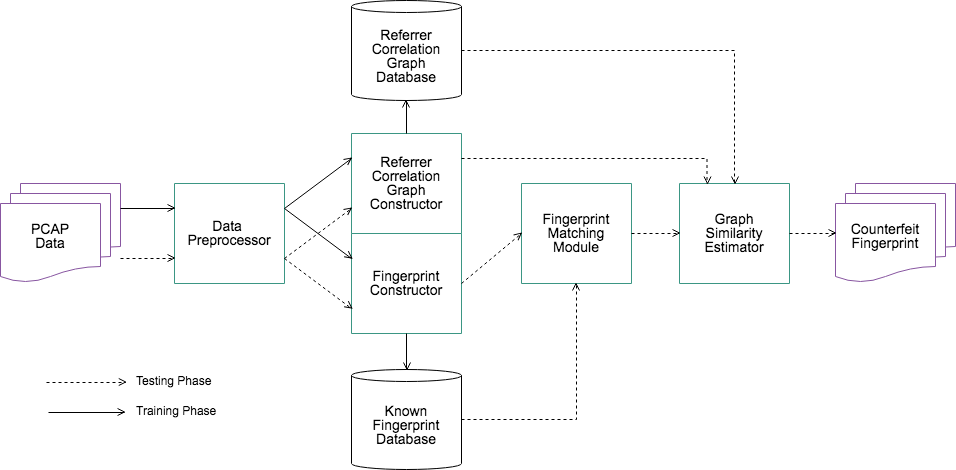
\includegraphics[width=400pt]{image/sa.png}
\caption{An overview of our counterfeit fingerprint detection system. Five subsystems are depicted: (1) data preprocessor subsystem, (2) fingerprint constructor subsystem, (3) fingerprint matching subsystem, (4) referrer correlation graph constructor subsystem, and (5) graph similarity estimator subsystem. The system only takes the PCAP files of outbound HTTP traffics as input. In training phase, subsystem (1) and (2) passively extract the benign fingerprint from an application's outbound HTTP traffic, and subsystem (3) could use fingerprints to classify benign traffic in the testing phase. We note that referrer correlation extraction in the subsystem (4) is a key step, in the sense that if it can extract discriminative features for counterfeit fingerprint detection, the detection in the subsystem (5) is relatively straightforward.}
\label{fig:sa}
\end{figure*}

\subsection{Data Preprocessor}

\subsection{Fingerprint Constructor}

\subsection{Fingerprint Matching Module}

\subsection{Referrer Correlation Graph Constructor}

\subsection{Graph Similarity Estimator}
\section{Experiment Results}

In this section, we would describe the datasets that we used to perform our experiments. For starting our experiments we have used two different datasets, simulated and real-world data. The simulated data is enable to evaluate the detection performance of our system and compare with DECANTeR \cite{bortolameotti2017decanter}.


\subsection{Experimental Settings}

\begin{table*}[!h]
\centering
\caption{Overview of the Datasets. We collect five datasets which industry series sets were real-world flows and the remaining of three were simulated data. Since the real-world traffic cannot be properly labeled, we treat real-world data as benign traffic. These data are captured by tcpdump and then using the scapy module to extract the HTTP header information we need.}
\label{tbl:db_02}
\begin{tabular}{|c|c|c|c|c|c|}
\hline\hline
Dataset         & Features & Types            & All Samples & Benign Samples & Malicious Samples \\ \hline
Industy\_flow01 & Packets  & Traffic Flows & 1,690,869   & 1,690,869  & N/A               \\ \hline
Industy\_flow02 & Packets  & Traffic Flows & 68,234   & 68,234   & N/A               \\ \hline
Dataset\_01     & Packets  & Botnet          & 1,444    & 1,094     & 350               \\ \hline
Dataset\_02     & Packets  & Botnet          & 1,342    & 1,102     & 240               \\ \hline
Dataset\_03     & Packets  & Botnet          & 1,045   &  877      & 168               \\ \hline\hline
\end{tabular}
\end{table*}


In the following, we briefly present the datasets we used for evaluation in our system. The dataset information is represented in table~\ref{tbl:db_02}.

\begin{itemize}

\item {\bf Real-world Data}

The outbound HTTP traffics we collect from more than hundreds of machines in a technology industry. Users of these machines include accountants, engineers, sales executive, and administrative personnel. Since the users vary from different occupations that lets data become various and complexity. The real world dataset has split into two sets, one is training and the other is testing. Training set has covered first few days and testing set is the traffics of last days. In training set, Industy flow\_01 contains 1,690,869 HTTP requests. and the testing set Industy flow\_02 contains 68,234 HTTP requests in this real-world dataset.

\item {\bf Simulated Data}

In this paper, our goal is a detection of counterfeit fingerprint which would pretend to be browser activities in outbound HTTP traffics. However, this kind of attack is secret and hidden penetration, and hard to collect in the real world. Therefore, we build a botnet malware and monitor its outbound HTTP traffics. As we know, early botnets generally used Internet Relay Chat (IRC) channel to communicate C\&C server. In recent years, botnets also start to communicate C\&C server through HTTP protocol. Furthermore, we need to build a botnet with the spoofing headers which can evade other detection systems. That is why we collect three different simulated botnet traffics. In Dataset\_01, it has no spoofing headers from infected host's outbound HTTP traffics. Dataset\_02 consists of the botnet traffics with simple spoofing, and which means our botnet sending the requests to web-like user agent through HTTP protocol. Finally, Dataset\_03 is totally modifying the headers information, and the malware investigates which browser is used by the user or host, and fills the field User-Agent with that specific browser. Moreover, it also fills up some common requests header fields, like Accept, Accept-Encoding, Accept-Language, and Referrer.

\end{itemize}

\subsection{Evaluation Metrics}

Essentially, Our system is a flow filter aim to identify the suspicious requests with the headers field. Four well-known metrics for evaluating the effectiveness of proposed method are adopted as followings: ``true positive''($TP$) means the number of normal requests which belong to normal traffic. ``False negative''($FN$) is the number of normal traffic and its results are wrongly predicted. Similarly, ``true negative''($TN$) means the number of abnormal traffic and the system predict it as malicious requests, while ``false positive''($FP$) is the number of abnormal traffic that the system predicts it as normal traffic. Based on the accumulation of $TP, FN, TN$, and $FP$, one extended metrics ($accuracy$) popularly used in machine learning problems are also adopted here to evaluate proposed method and listed in equations below. Note that the optimal $accuracy$ of $1.0$ means all of the malware are successfully picked out by the proposed approach. 


\begin{eqnarray}
\label{eq:accuracy}
Accuracy = \frac{TP+TN}{TP+TN+FP+FN}
\end{eqnarray}

\subsection{Effectiveness Analysis}

\begin{table*}[!h]
\centering
\caption{Overview of Evaluation.
For testing the robustness, we add the real-world traffic into each simulated data. We compare the performance of our system and DECANTeR\cite{bortolameotti2017decanter} against different data sets. The accuracy is calculated by equation (\ref{eq:accuracy}) and the detail result will show below.}
\label{tbl:db_03}
\begin{tabular}{|c|c|c|c|c|c|c|c|c|}
\hline\hline
\multirow{2}{*}{Dataset}                     & \multirow{2}{*}{System} & \multirow{2}{*}{HTTP Requests} & \multicolumn{4}{c|}{Evaluation Metrics} & \multirow{2}{*}{Accuracy} & \multirow{2}{*}{\begin{tabular}[c]{@{}c@{}}Counterfeit Fingerprint\\ Detection Rate\end{tabular}} \\ \cline{4-7}
                                             &                         &                                & TP         & TN      & FP      & FN     &                           &                                                                                                   \\ \hline
\multirow{2}{*}{Dataset\_01+Industy\_flow02} & DECANTeR \cite{bortolameotti2017decanter}                & \multirow{2}{*}{69,678}        & 69,328     & 350     & 0       & 0      & 1.0000                    & N/A                                                                                               \\ \cline{2-2} \cline{4-9} 
                                             & Our System              &                                & 69,328     & 350     & 0       & 0      & 1.0000                    & N/A                                                                                               \\ \hline
\multirow{2}{*}{Dataset\_02+Industy\_flow02} & DECANTeR  \cite{bortolameotti2017decanter}               & \multirow{2}{*}{69,576}        & 69,336     & 240     & 0       & 0      & 1.0000                    & N/A                                                                                               \\ \cline{2-2} \cline{4-9} 
                                             & Our System              &                                & 69,336     & 240     & 0       & 0      & 1.0000                    & N/A                                                                                               \\ \hline
\multirow{2}{*}{Dataset\_03+Industy\_flow02} & DECANTeR   \cite{bortolameotti2017decanter}              & \multirow{2}{*}{69,279}        & 69,109     & 0       & 168     & 2      & 0.9975                    & 0\%                                                                                               \\ \cline{2-2} \cline{4-9} 
                                             & Our System              &                                & 69,109     & 168     & 0       & 2      & 0.9999                    & 100\%                                                                                             \\ \hline\hline
\end{tabular}
\end{table*}



Just as we know, malware can easily modify the HTTP header, therefore, we build three kind of malware to evaluate our approach. With these botnets, they all have the same purpose, and which would steal some sensitive information (such as OS information, system account, and the password) and send requests to the C\&C server periodically waiting for commands to execute. The difference between them is the degree of the spoofing HTTP headers. The botnet in Dataset\_01 doesn't spoof any HTTP headers, and we fill up with the empty to the User-Agent field. The botnet in datset\_02 only simply sets the User-agent as a common browser which calls Internet Explore (IE). In the Dataset\_03 , botnet would specifically detect the victim's browser version and system language, and then fill them into the HTTP header. In addition, for the reference field in a HTTP header that we point to the default website. For testing system's robustness, we merge dataset Inudstry\_flow 02 to each simulated data. It may greatly increase the complexity of the detection task. The result is shown in table~\ref{tbl:db_03}, we can see that our system and DECANTeR \cite{bortolameotti2017decanter} both have the great performance with Dataset\_01 and Dataset\_02. However, we can notice that our system has a better performance for botnets in Dataset\_03 based on advanced spoofing methods. Since we calculated the distance of referrer correlation graph between the dataset and the training set. We use this method to find out the traffic that suspected counterfeit HTTP header fields. For the distance we will give a threshold, this threshold will affect the false positive rate and the detection rate of counterfeit HTTP header. We set the threshold as "10" in this dataset.

In the training stage, We build each fingerprint through the clean data for both systems. For with no User-Agent request headers, which filled in '-' in User-Agent field, we will use the domain and IP to create the fingerprints. Moreover, this concept is just like the idea of the whitelist, and malware can't evade our system detection through the settings of HTTP header with empty User-Agent. The result shows that two detection systems both got an excellent performance in the Dataset\_01. Some malware would use a web-like User-Agent to camouflage themselves as a browser to avoid the system detection. In Dataset\_02, the malware would modify the HTTP header field User-Agent to IE, and disguise itself as a browser and communicate with C\&C server. For this validation set, both systems also got a good score when a malware disguises itself as a browser, and our system would firstly check the request whether whitelist has this fingerprint or not. If yes, the system will compare the difference with these fingerprints. So, unless the malware can guess or use some advanced technology to get the browser information and the language of the OS system used by the victim, and then using this information to forge the HTTP header fields. Otherwise, it is not easy to avoid the first stage of our detection system.

For advanced spoofing methods, the malware can detect the victim's system information such as browser version and system language, and then malware would modify the HTTP header fields when sending requests to C\&C server. For this reason, it is not robust with only the first phase of detection (e.g., DECANTeR \cite{bortolameotti2017decanter}, DUMONT \cite{schwenk2011adaptive}, and WebTap \cite{borders2004web}). Therefore, in addition to creating the fingerprints, we also established the referrer correlation graph during the training phase. For the traffic with the labeling as normal through the first phase by the detection system, and we can carry out the second phase of detection, the detection system would compare the graph edit distance between each referrer correlation graphs. The idea of this detection stems from the fact that we think when humans are browsing the websites, they would click the hyperlink to where they want to browse, and these referrers of the requests can be generated as a referrer correlation path. On the other hand, malware that disguised as a browser cannot link out such a path. We apply this concept to use GED to calculate the difference between these referrer correlation graphs. The results show that our approach is better than DECANTeR \cite{bortolameotti2017decanter}, and it could detect the malware sending requests in Dataset\_03 which using advanced spoofing methods to evading detection system.

\subsection{Limitation and Future Work}

There are two main problems in our approach, however, they are infrequent in practice. First problem is the duration of model training or fingerprint constructing that need a non-compromised environment. Because, our approach is an extension of DECANTeR \cite{bortolameotti2017decanter}, and which needs to generate an application's fingerprint for anomaly detection in a clean environment. Therefore, we also have to perform our approach at the same scenario for benign fingerprint and correlation model construction. The second problematic situation may happen (e.g., TLS) that is due to a lack of browser referrer contents, and this situation may difficultly construct a referrer correlation graph. Moreover, we couldn't extract any information from an encrypted PCAP file when it was encapsulated in TLS unless we use a TLS proxy for traffic decryption. Fortunately, this could be resolved by a tool (e.g., Burp Suite) for interception of TLS requests. 

In the further work, the counterfeit fingerprint not only appears in browser network activities but also usually used in background application for evading detections, and which is breifly described in DECANTeR \cite{bortolameotti2017decanter}. Therefore, we will resolve counterfeit fingerprint in each background application based on the same idea concept with this paper in the future.

\section{Conclusion}
\section*{Acknowledgment}

This research is supported in part by the Ministry of Science and Technology of Taiwan under grants number MOST-105-2221-E-011-085-MY3. The authors also gratefully acknowledge the helpful comments and suggestions of the reviewers, which have improved the contributions of this paper.


\bibliographystyle{IEEEtran}
\bibliography{IEEEtranBST2/IEEEexample}

\end{document}
